\documentclass{article}

%used package
\usepackage[]{graphicx}
\usepackage[utf8]{inputenc}
%package for code
\usepackage{listings}
\usepackage{wrapfig}

% Adds hyperlinks to references
\usepackage{hyperref}

\usepackage[italian]{babel}

% If multiple images are to be added, a folder (path) with all the images can be added here 
\graphicspath{{images/}}

\usepackage[left=80pt,right=80pt]{geometry}

\usepackage{xcolor}
 
\lstdefinestyle{mystyle}{
    keywordstyle=\color{blue},
    stringstyle=\color{blue},
}

\lstset{style=mystyle}

\begin{document}

%Adds the title page
\begin{titlepage}
	\centering
	{\large Laboratorio di Reti - Corso A \par}
	\vspace{1.5cm}
	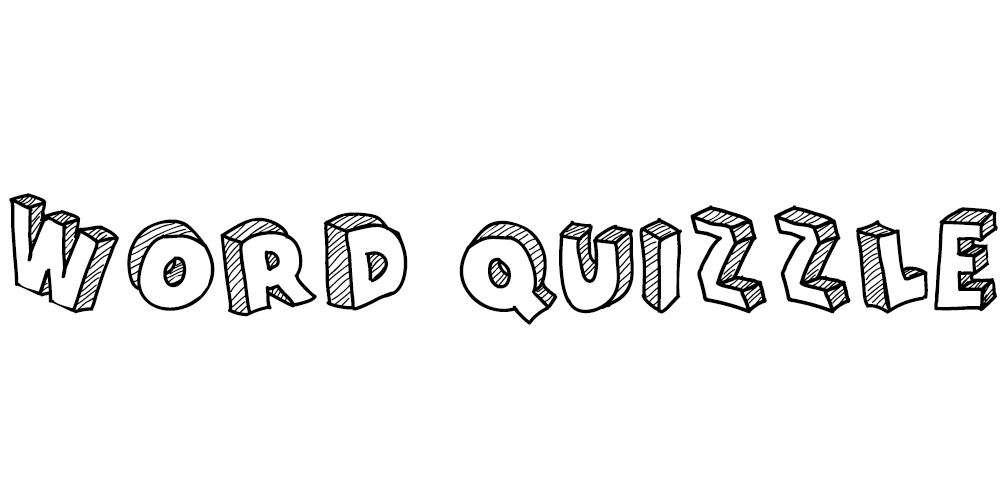
\includegraphics[scale=0.3]{quizzlelogolong.png} \\
	{\large \textbf{documentazione riguardante scelte implementative e protocollo messaggi} \par}
	\vspace{4cm}
	{\large Docente: Laura Ricci \\
	        Studente: Raffaele Apetino, Matricola 549220 \par}
	\vspace{1.3cm}

    
\includegraphics[scale=1]{universitapisa.png}
    
    \vspace{1.3cm}
    
	% Information about the University
	{\normalsize Dipartimento di Informatica \par}
		
	% Set the date
	{\normalsize 30-01-2020 \par}
	
	\pagebreak

\end{titlepage}

% Adds a table of contents
\tableofcontents{}
\clearpage

\section{Introduzione}
Il progetto riguarda la programmazione di un sistema di sfide di traduzione (italiano-inglese) utilizzando il linguaggio Java. E' richiesto anche di gestire una rete sociale in cui gli utenti possono registrarsi, aggiungere amicizie e confrontarsi attraverso classifiche basate sul punteggio. La registrazione degli utenti avviene tramite Remote Method Invocation. Mentre il dialogo tra client e server secondo connessione TCP (che chiameremo TCP standard). La sfida sfrutta anch'essa il protocollo TCP (TCP sfida). Per le notifiche di sfida tra due utenti è stato richiesto di usare UDP. Le traduzioni si basano sulla API offerta dal servizio gratuito \href{https://mymemory.translated.net/doc/spec.php}{MyMemory}. \\
L'interfaccia grafica è stata creata sfruttando il framework \href{https://docs.oracle.com/javase/8/javafx/get-started-tutorial/jfx-overview.htm}{JavaFX} e l'applicativo \href{https://gluonhq.com/products/scene-builder/}{SceneBuilder} che permette la creazione di file FXML \footnote{an XML-based user interface markup language created by Oracle for defining the user interface of a JavaFX application} attraverso semplici drag and drop, crop e resize dei vari elementi che compongono l'interfaccia. I file FXML in output sono poi caricabili tramite classi apposite di JavaFX come la classe FXMLLoader. Per la gestione dei file di persistenza, contenenti le informazioni delle strutture dati del server, ho utilizzato il formato JSON con l'aiuto delle librerie \href{https://code.google.com/archive/p/json-simple/}{JSON.simple} e \href{https://github.com/google/gson/blob/master/UserGuide.md}{Gson} (Google).

\section{Istruzioni per Compilazione e Avvio}
Il progetto è stato testato su ambienti MacOS e Linux (Ubuntu). Utilizzare per la compilazione del client un JDK dalla versione 8 alla 11 (esclusa) poichè contiene nativamente JavaFX. Nel caso in cui si utilizzasse un JDK 11 o maggiore è nesessario scaricare i moduli aggiuntivi di JavaFX dal seguente link: \href{https://gluonhq.com/products/javafx/}{https://gluonhq.com/products/javafx/}. \newline 


Compilazione ed esecuzione Server:
\begin{lstlisting}[
    basicstyle=\small,
    language=bash
    ]
Compilazione:

Spostarsi all'interno della directory WordQuizzle/WQServer
javac -cp ".:../jars/json-simple-1.1.jar:../jars/gson-2.8.6.jar:" WQServer.java

Esecuzione:

Nella directory WordQuizzle/WQServer
java -cp ".:../jars/json-simple-1.1.jar:../jars/gson-2.8.6.jar:" WQServer
\end{lstlisting}
\clearpage
Compilazione ed esecuzione Client:
\begin{itemize}
\item JDK da 8 a 11 (escluso):
\begin{lstlisting}[
    basicstyle=\small,
    language=bash
    ]
Compilazione:

Spostarsi all'interno della directory WordQuizzle/WQClient
javac -cp ".:../jars/json-simple-1.1.jar:../jars/gson-2.8.6.jar:" WQClient.java

Esecuzione:

Nella directory WordQuizzle/WQClient
java -cp ".:../jars/json-simple-1.1.jar:../jars/gson-2.8.6.jar:" WQClient
\end{lstlisting}
\item JDK da 11 o superiore:
\begin{lstlisting}[
    basicstyle=\small,
    language=bash
    ]
Compilazione:

Copiare l'archivio zip dei moduli scompattato nella cartella jars
Spostarsi all'interno della directory WordQuizzle/WQClient
javac -cp ".:../jars/json-simple-1.1.jar:../jars/gson-2.8.6.jar:" 
--module-path ../jars/javafx-sdk-**/lib/ --add-modules ALL-MODULE-PATH WQClient.java

(fare attenzione e inserire la versione del proprio sdk)

Esecuzione:

nella directory WordQuizzle/WQClient
java -cp ".:../jars/json-simple-1.1.jar:../jars/gson-2.8.6.jar:" 
--module-path ../jars/javafx-sdk-**/lib/ --add-modules ALL-MODULE-PATH WQClient

(fare attenzione e inserire la versione del proprio sdk)
\end{lstlisting}
\end{itemize}

\clearpage

\section{WQServer}
Il server appena avviato si occupa di creare l'istanza del WQDatabase (o ricrearla partendo dai file di persistenza). In seguito, dopo aver creato ed esportato il registry per la registrazione tramite RMI, si mette in ascolto sulla socket in un ciclo dove accetta i vari client che vogliono connettersi ad esso. Per limitare il numero di client collegati, il server sfrutta un Thread Pool Executor con LinkedBlockingQueue. Questo permette di porre un limite al numero massimo di thread che una singola macchina può gestire, evitando così la creazione di infiniti thread ed di conseguenza il collasso della macchina. Dopo l'accettazione del client sulla socket viene eseguito un WQTask che si occuperà di quel singolo client fino al momento di logout dell'utente. Se la pool è al completo il client aspetta nella coda.

% A  after the section/chapter command indicates an unnumbered header which will not be added to the table of contents
\subsection{Protocollo di comunicazione standard}
La sintassi dei messaggi inviati dal client al server della comunicazione TCP standard è così definita: (differisce dal protocollo TCP sfida)

\begin{table}[h]
\centering
\begin{tabular}{l|l|l|l|l}
LOGIN  & USERNAME   & PASSWORD   & HOSTADDRESS & UDPPORT  \\
ADD    & USERNAME   & NICKFRIEND &             &          \\
REMOVE & USERNAME   & NICKFRIEND &             &          \\
POINTS & USERNAME   &            &             &          \\
LIST   & USERNAME   &            &             &          \\
RANK   & USERNAME   &            &             &          \\
CHALL  & CHALLENGER & CHALLENGED &             &          \\
LOGOUT & USERNAME   &            &             &         
\end{tabular}
\end{table}

Si noti che la registrazione non è presente perchè avviene tramite RMI.

\subsubsection{Codici di Errore}
Codici inviati dal Server al Client sotto connessione TCP standard.
\begin{table}[h]
\centering
\begin{tabular}{l|l}
9  & Operazione non valida                 \\
10 & Registrazione OK                      \\
11 & Username già presente                 \\
12 & Login OK                              \\
13 & Password Errata                       \\
14 & Utente Inesistente                    \\
15 & Utente già online                     \\
16 & Logout OK                             \\
17 & Già presente nella lista di amicizie  \\
18 & Aggiunto amico                        \\
19 & Non presente nella lista amicizie                     \\
20 & Rimozione amicizia OK                 \\
21 & Invio richiesta sfida                 \\
22 & Utente non online                    
\end{tabular}
\end{table}

\subsection{WQTask}
Ad ogni client è associato un WQTask apposito che gestirà tutte le sue richieste. Consiste in un ciclo che legge sequenzialmente le richieste del client arrivate secondo protocollo e le tokenizza. Ad ogni richiesta il thread chiama i rispettivi metodi di WQDatabase, classe definita per gestire tutti i dati. 

\subsection{WQDatabase}
E' la classe cardine del server e in essa sono contenute le strutture dati che memorizzano tutte le informazioni dei giocatori. Attraverso i metodi di questa classe è possibile aggiornare i file e gli attributi dei giocatori. Le due strutture principali sono:
\begin{lstlisting}[language=Java]
private HashMap<String, String> passwords;
private HashMap<String, WQUser> users;
\end{lstlisting}
La prima è una HashMap che utilizza come chiave il nome utente e come valore la password salvata tramite hashing one-way SHA-256 concatenando username e password. Questo permette maggiore sicurezza nel caso in cui il file di persistenza "passwords.json" venga raggiunto da chi non è autorizzato. Il concatenamento dell'username e della password permette di ottenere due immagini hash diverse nell'eventualità che due utenti scelgano la stessa password. \\
La seconda struttura invece si occupa di tenere in memoria tutti gli utenti del gioco. Ha come chiave il nome utente e come valore una istanza di WQUser (definito nella prossima sottosezione). 
Il metodo costruttore di WQDatabase si occupa, nel caso in cui i file di persistenza siano già presenti, di ricreare tutte le istanze delle due strutture sfruttando la libreria Gson. I file di persistenza vengono aggiornati qualora un utente si registri, aggiunga o rimuova un amico e quando i punti dell'utente cambiano. Questa scelta può risultare computazionalemte costosa ma sicura nell'eventualità di crash da parte del server, poichè i dati rimarranno consistenti. Una soluzione alternativa potrebbe essere la creazione di un thread apposito che periodicamente si occupi di aggiornare i file JSON.

\subsection{WQUser}
Classe che si occupa di rappresentare gli utenti/giocatori di WordQuizzle. In essa sono contenute le variabili per salvare l'indirizzo IP del client, la porta UDP per le notifiche, il punteggio, lo stato (online/offline) e la lista delle amicizie. Quest'ultima è definita come un ArrayList di stringhe (username). Per ottenere quindi le informazioni degli amici è necessario eseguire una ricerca nella HashMap "users" con chiave username (costo 0(1) * O(dimLista)). La classe implementa Comparable, poichè gli utenti dovranno essere confrontati secondo la variabile contentente i punti, per poter creare la classifica.

\section{WQClient}
Il client è composto principalmente da due thread. Un thread si occuperà delle notifiche UDP, mentre il thread principale avvia l' interfaccia grafica chiamando il metodo launch() definito da JavaFX (notare come WQClient estenda Application, classe definita da JavaFX). Il metodo launch() chiamerà a sua volta il metodo start() che si occuperà di creare lo "stage". Viene poi caricato il file FXML della scena di login usando FXMLLoader ed infine viene associato il controller della scena (RegisterLoginController). L'interfaccia grafica da questo momento in poi itera attraverso le varie "scene" dalla schemata principale (con controller MainViewController) a quella del gioco (GameViewController). "A controller is a compiled class that implements the "code behind" the object hierarchy defined by the document." \cite{javafxDocumentation} Il compito del Controller è quindi quello di associare ogni "ID" (associazione tra controlli della GUI e ID avviene tramite SceneBuilder) e il codice che deve essere eseguito quando l'evento occorre (ad esempio click su un tasto). Tutti i controller hanno un riferimento alla classe WQClient, in essa sono definiti tutti i metodi "handler" che si occupano di comunicare con il server tramite socket TCP standard.

\subsection{RegisterLoginController}
\begin{center}
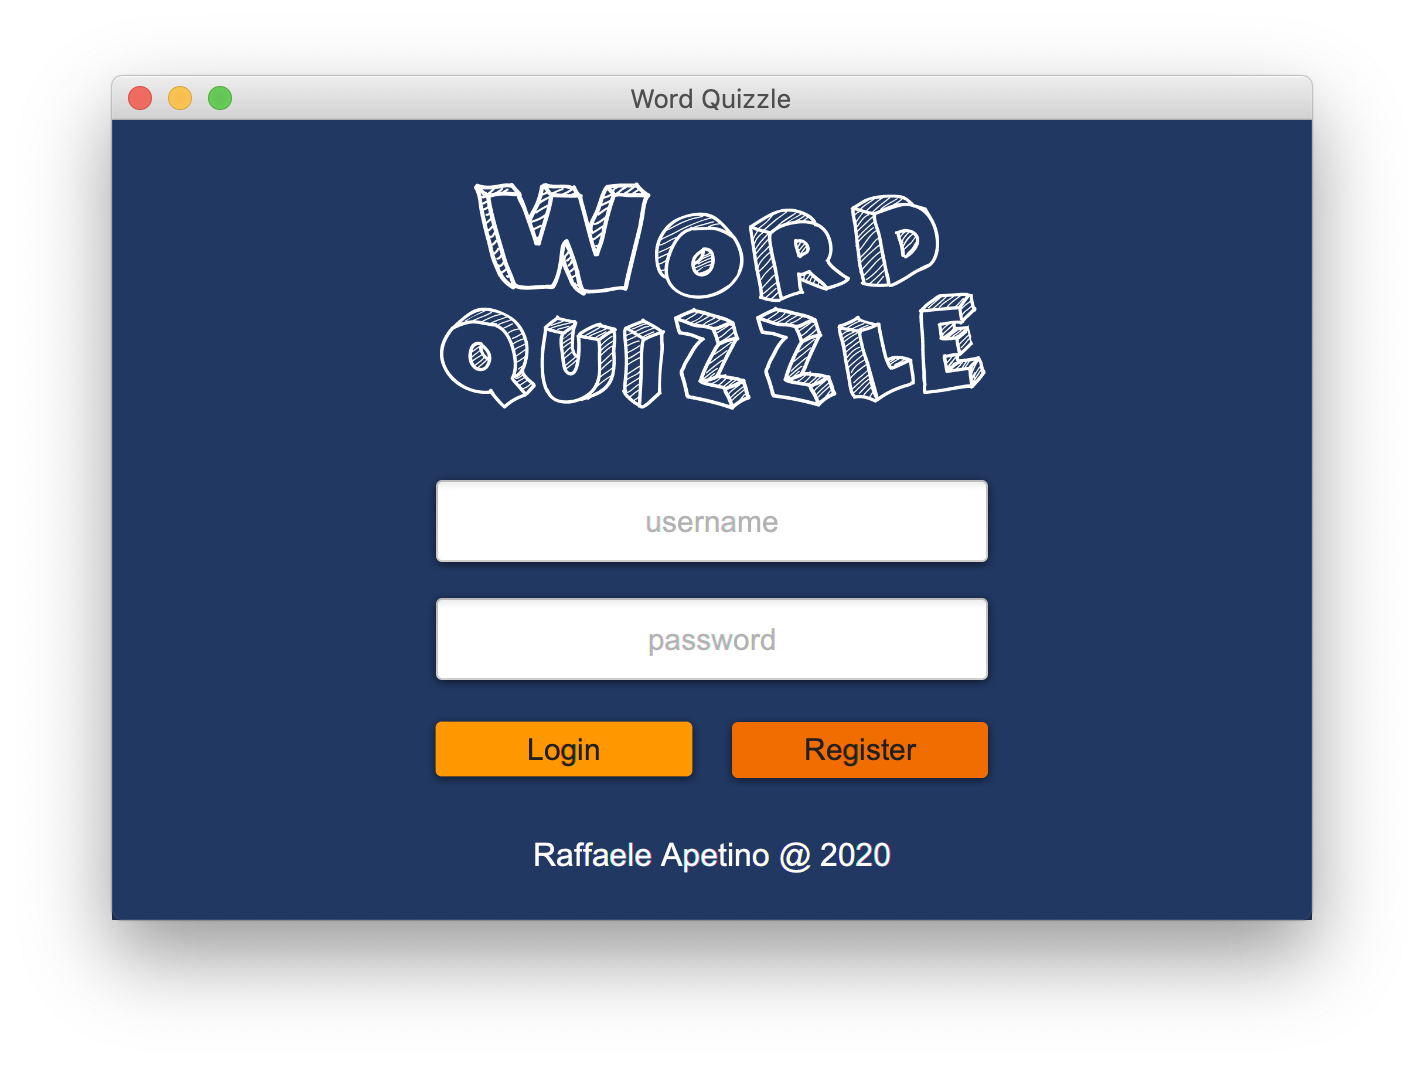
\includegraphics[scale=0.5]{quizzleloginregister.png}
\end{center}
Il controller per la registrazione e il login contiene due "TextField", una "Label" e due "Button". Le TextField sono passive, cioè non fanno parte di quegli elementi che generano eventi. Per gestire l'evento di "OnClick" dei due bottoni ho definito due metodi:
\begin{itemize}
    \item registerbtnAction: gestisce il tasto di registrazione, chiama il metodo RMI della registry passando come parametri i due campi delle TextField.
    \item loginbtnAction: gestisce il tasto di login, chiama il metodo login\textunderscore handler di WQClient passando come parametri i due campi delle TextField. Il metodo login\textunderscore handler si occupa di creare un collegamento TCP con il server per poi inviare la stringa di login secondo protocollo di comunicazione standard. Se il login è corretto, crea la socket UDP e manda in esecuzione il thread che si occuperà di ricevere le notifiche di sfida. (Tutto ciò che riguarda la sfida e notifiche è descritta nel capitolo Sfida). 
\end{itemize}
In caso di errore, sia per il login che per la registrazione, viene aggiornata la Label (posizionata sotto i due tasti) con la stringa associata al codice di errore.

\subsection{MainViewController}
\begin{center}
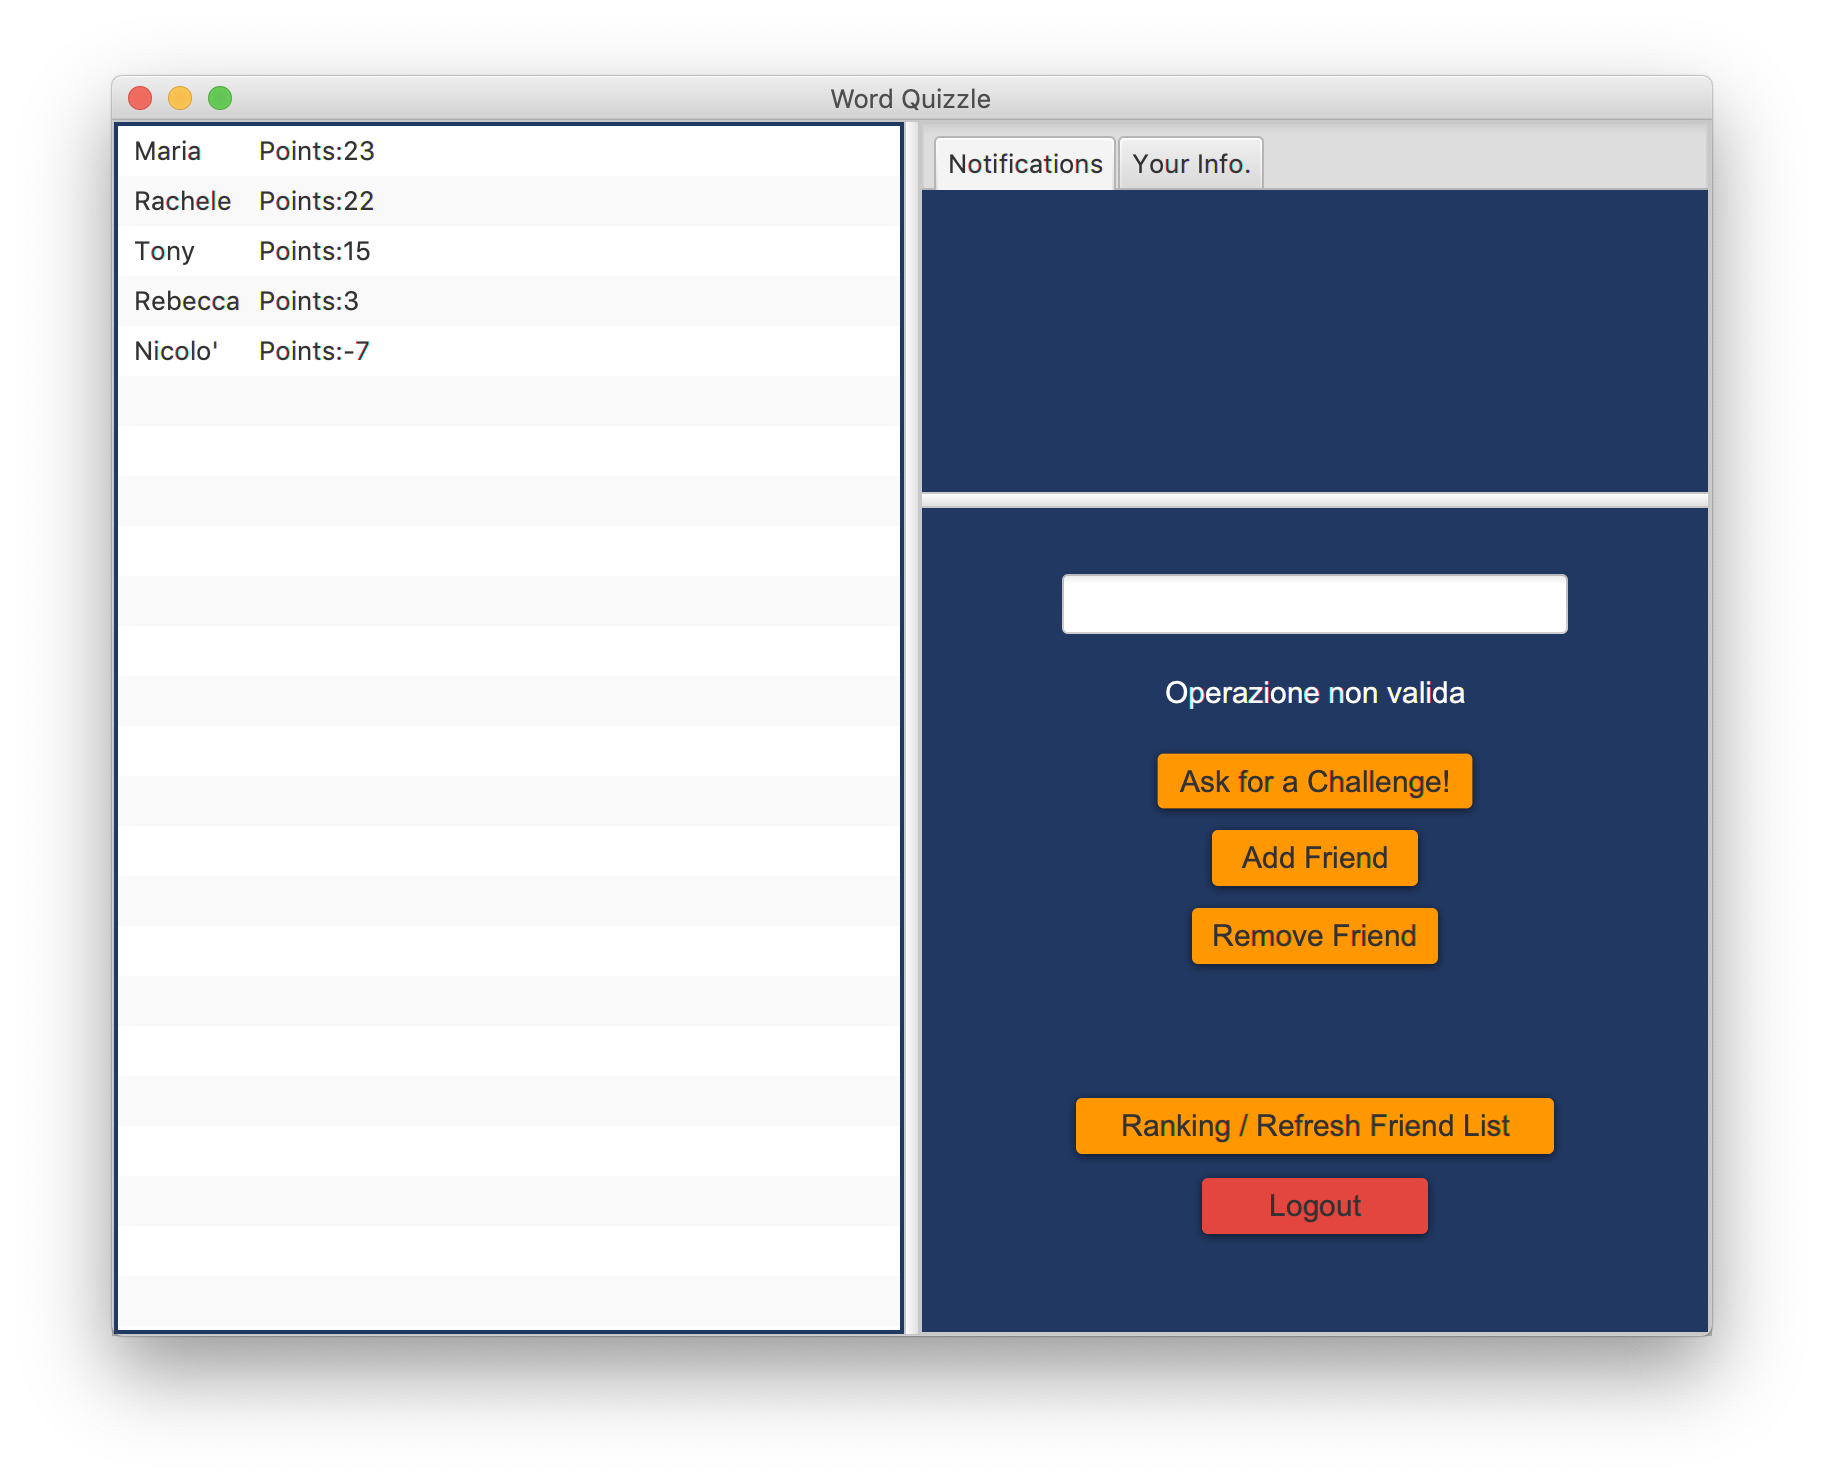
\includegraphics[scale=0.5]{quizzlemain.png}
\end{center}
La scena della schermata principale è divisa in due parti. Nella parte sinistra è presente una ListView di amici che possono essere aggiunti o rimossi grazie alla TextField e ai bottoni presenti nella parte di destra. La ListView può essere settata in modalità classifica o lista di amicizie cliccando sul Toggle apposito. Sono presenti due Tab, una per le notifiche e una contenente le informazioni correnti dell' utente (username e punteggio).
Ogni Button si occupa di chiamare il metodo "handler" associato definito in WQClient. Il metodo "handler" invia al server i comandi seguendo il protocollo e nel caso di errore aggiorna la Label di errore posizionata sotto alla TextField.
\clearpage

\section{Sfida}
Prima di illustrare la sfida è bene definire il thread che gestisce le notifiche lato client.

\subsection{WQNotify}
E' una classe client-side che si occupa di gestire tutte le notifiche che arrivano tramite UDP. Il thread viene fatto partire appena il client è riuscito a loggarsi con successo, passandogli come parametro la DatagramSocket creata dal thread che gestisce l'interfaccia grafica. L' istanziazione della socket nel thread principale mi permette di poter eseguire la socket.close() quando il client esegue il logout, affinchè si possa catturare l'eccezione e terminare il processo. Il thread è bloccante sulla receive della socket. Il suo principale compito è quello aggiungere ad una LikedList le notifiche in politica FIFO, rendere visibile o invisibile la tab delle notifiche e associare alla notifica l'username dello sfidante (ricevuto all'interno del datagramma).

\subsection{Protocollo Notifica}
\begin{wrapfigure}{l}{6cm}
\centering
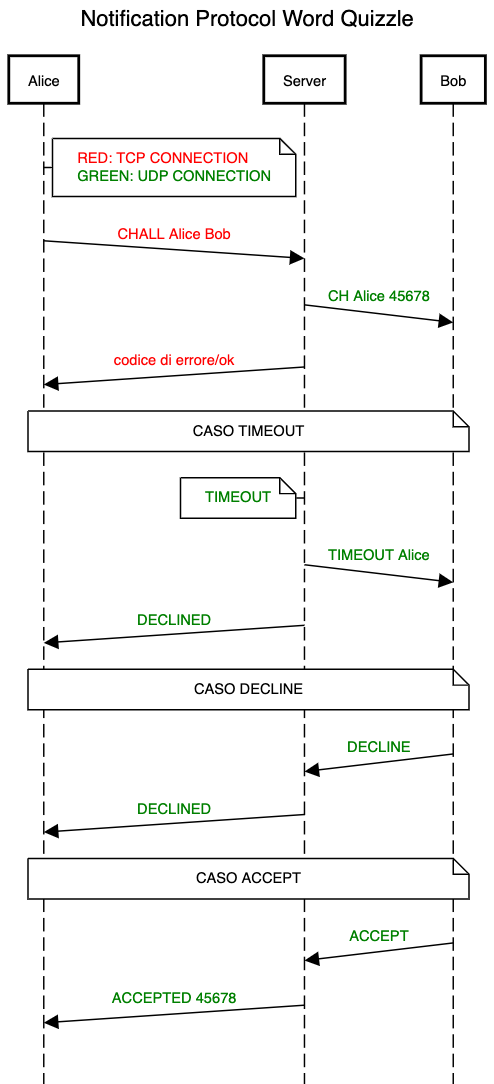
\includegraphics[width=6cm]{chprotocolscheme.png}
\end{wrapfigure}
Il protocollo di notifica ha inizio quando Alice manda a Bob, sotto connessione TCP standard, il messaggio "CHALL Alice Bob" che segue il protocollo di comunicazione standard. Il server riceve il messaggio, quindi lancia il thread della sfida creando una nuova socket TCP su una porta creata randomicamente (la chiameremo TCPport). Successivamente il server invia tramite UDP allo sfidato (Bob) il messaggio "CH Alice TCPport". Se l'invio della notifica è avvenuto con successo o ha riscontrato errori il server avvisa Alice tramite socket TCP standard. Il client di Bob, ricevuto il messaggio di sfida, aggiunge in coda alla LinkedList la notifica e aggiorna l'interfaccia grafica.
Ci possiamo trovare quindi in 3 situazioni:
\begin{enumerate}
  \item Bob non risponde alla richiesta di sfida: la socket UDP del server non riceve risposta entro il tempo T1 e scatta il timeout. Il server invia "TIMEOUT username" in un datagramma a Bob, che si occuperà di rimuovere la notifica dalla lista. Mentre invia ad Alice "DECLINED" tramite UDP, il client di Alice si occuperà di aggiornare la Label di errore e riattivare il tasto di richiesta di sfida.
  \item Bob non accetta la sfida: Bob invia il messaggio "DECLINE" al server e aggiornata la sua GUI rimuovendo la notifica. Il server ricevuto il datagramma di Bob avvisa Alice inviando "DECLINED" in un altro datagramma.
  \item Bob accetta la sfida: Bob invia al server "ACCEPT", in seguito il server spedisce ad Alice "ACCEPTED TCPport". Notare come Alice non era ancora a conoscenza della TCPport associata alla sfida.
\end{enumerate}
\clearpage
Una volta accettata la sfida da parte di entrambi i giocatori, i rispettivi client eseguono una chiamata al metodo gotoGame() di WQClient, caricando la scena principale del gioco (GameView.fxml).

\subsection{Protocollo Sfida}
Messaggi inviati dal Server al Client:

\begin{table}[h]
\centering
\begin{tabular}{lllll}
parola\textunderscore ita  & var\textunderscore double \\
CHEND & punti\textunderscore ottenuti & parole\textunderscore corrette & parole\textunderscore errate & esito\textunderscore sfida \\
TIMEOUT & punti\textunderscore ottenuti & parole\textunderscore corrette & parole\textunderscore errate & esito\textunderscore sfida \\
\end{tabular}
\end{table}
\hfill \break
Messaggi inviati dal Client al Server:
\begin{table}[h]
\centering
\begin{tabular}{ll}
username & word\textunderscore eng \\
CHEXITED & \\
\end{tabular}
\end{table}

\subsection{WQChallenge on Server}
La classe WQChallenge rappresenta il thread dedicato alla sfida, viene lanciato dal thread la server che gestisce lo sfidante. Fa utilizzo del selector, è quindi un singolo thread che gestisce sequenzialmente entrambi i client (sfidato e sfidante). Il thread appena lanciato si occupa di scegliere randomicamente le K parole italiane dal file JSON "words.json", imposta la socket TCP in modalità non bloccante e si posiziona in ascolto sulla select(). \\
Appena uno dei due client si collega, questo implica che la sfida è stata accettata, il thread si occupa di chiamare il servizio API di traduzione singolarmente per ogni parola italiana. La chiamata al servizio REST avviene sfruttando la classe HttpsURLconnection e settando il metodo di richiesta a "GET". La risposta è una stringa JSON da analizzare con JSONParser fino a trovare la chiave "translatedText" che contiene come valore la traduzione più appropriata della parola italiana inviata. \\
Subito dopo aver tradotto le K parole parte il timer della sfida (WQChallTimer). Il timer fa utilizzo della classe Timer e TimerTask definite in Java. Il loro compito è quello di eseguire un task (RemindTask) non appena il tempo impostato è trascorso. Il task si occupa semplicemente di incrementare una variabile volatile atomica (timeover) per notificare al thread del selector che la sfida è terminata.
\\
La chiave associata alla socket del client è impostata in OP\textunderscore WRITE subito dopo l'accettazione. Inoltre alla key viene allegata una istanza di WQWord (definita nella prossima sottosezione). 

Se la chiave selezionata si trova in modalità scrittura viene inviata la parola italiana seguita da un valore "double", quest'ultimo è necessario al client per poter aggiornare la barra di avanzamento dell'interfaccia grafica.
Nell'ipotesi in cui uno dei due client termini (quindi la variabile volatile atomica endusers = 1) oppure le parole siano terminate (quindi l'indice contenuto nell'istanza di WQWord è maggiore K) o ancora nel caso in cui il timer sia scaduto (variabile atomica intera timeover = 1) il server invia il resoconto finale della sfida secondo protocollo di sfida.

Se la chiave selezionata è in modalità lettura, il server legge la stringa inviata dal client e la analizza. Se il payload corrisponde a "CHEXITED", significa che il client è uscito volotariamente dalla sfida, incrementa la variabile endusers e cancella la chiave dal selector. Se così non fosse, chiama il metodo "checkWords()" che si occupa di controllare la correttezza della traduzione, aggiornando inoltre il puteggio dell'utente nel database principale e nella struttura delle statistiche associata alla chiave. Il server considera la situazione in cui uno dei due client abbia terminato per primo (endusers = 1) non attribuendo punti per le parole inviate dall'ultimo client rimanente.

Al termine della sfida, dopo aver inviato entrambi i messaggi di esito, il thread si occupa di aggiornare i punteggi anche sui file di persistenza.

\subsubsection{WQWord}
Di fondamentale importanza è la classe WQWord definita per poter aggiungere in allegato alla key (chiave del selector) le informazioni necessarie per identificare il client che sta giocando. La classe contiene l'indice della parola da inviare e una classe ausiliaria "Statistics" necessaria per il calcolo delle statistiche finali della singola partita.

\subsection{GameViewController on Client}
\begin{center}
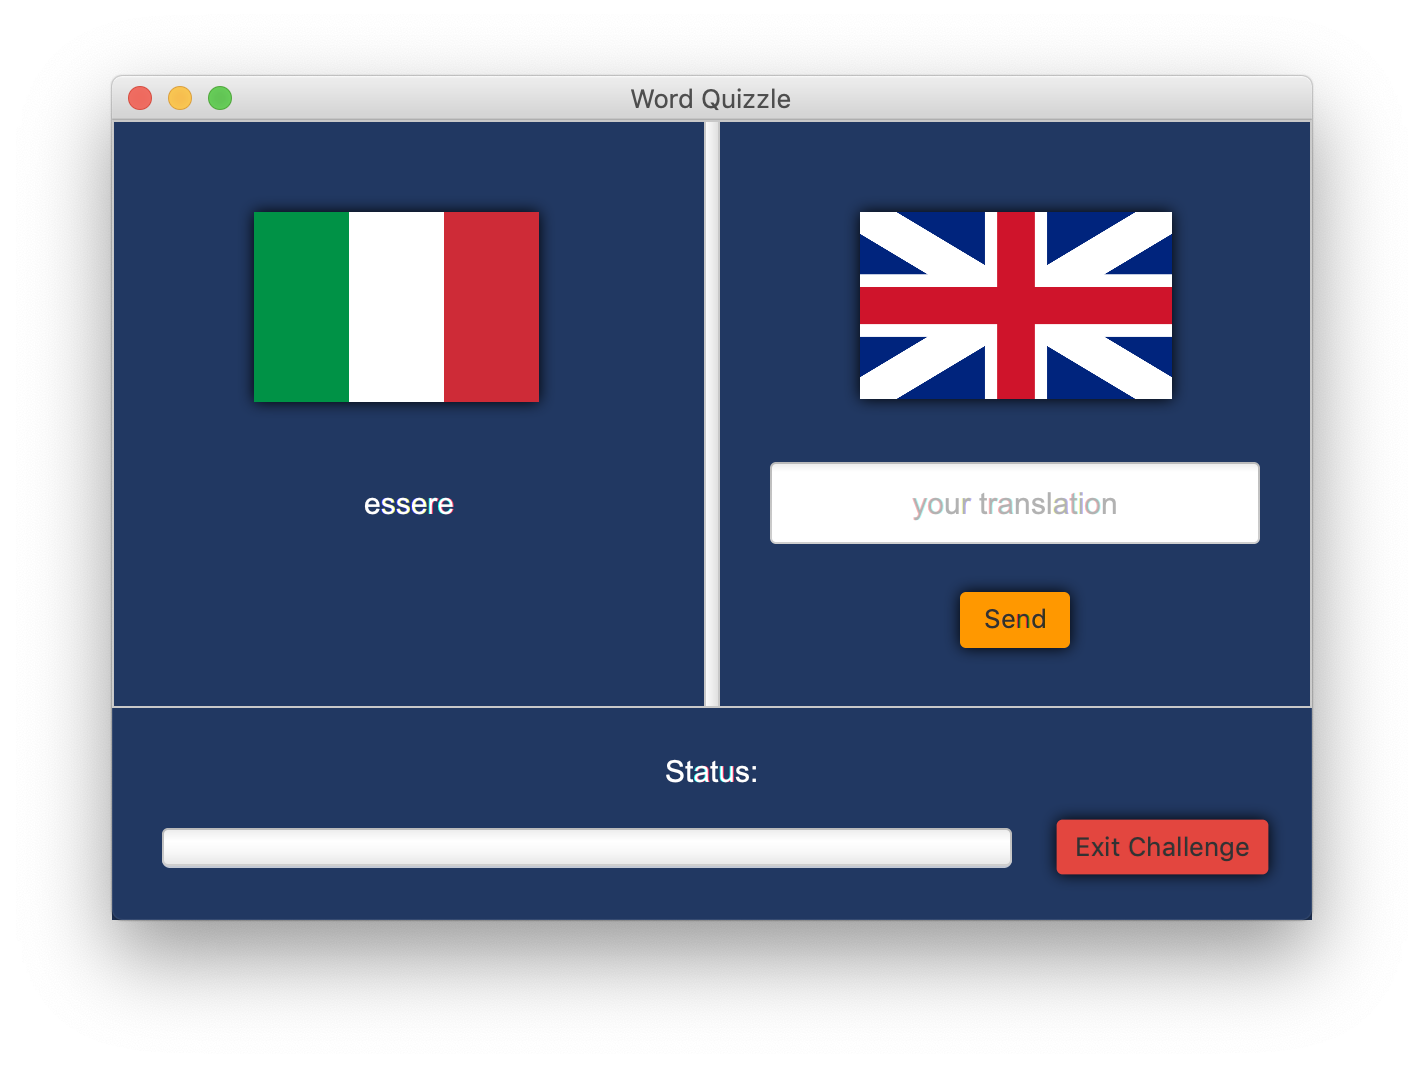
\includegraphics[scale=0.5]{quizzlegame.png}
\end{center}
Il Controller che si occupa del gioco è rappresentabile come una FSM con due stati: lettura e scrittura. Si trova inizialmente nello stato di lettura, subito dopo aver effettuato la connessione TCP al server sulla porta della sfida. Passa nello stato di scrittura non appena viene premuto il tasto di invio della parola e dopo l'invio del messaggio sulla socket TCP sfida, torna nello stato di lettura. 
Se il payload letto coincide con "CHEND" oppure "TIMEOUT" la sfida è terminata, quindi aggiorna l'interfaccia grafica con l'esito finale. Il client a questo punto attende che l'utente esca dalla sfida tramite l'apposito tasto. All'uscita il client spedisce "CHEXITED" ed infine imposta la scena della schermata principale.

% Adding a bibliography if citations are used in the report
\bibliographystyle{plain}
\bibliography{bibliography}

\end{document}
